\section{Models for Density (Mean)}

We considered modeling the response variable mean TCT. Previously, we considered median TCT. We took an identical approach to the previous models. That is, we first created a simple linear model for predicting the response mean TCT. That is, we created a model l.one.line.mean that only considers Log2(Biomass) as a predictor.

\vspace{12pt}



\begin{figure}[H]
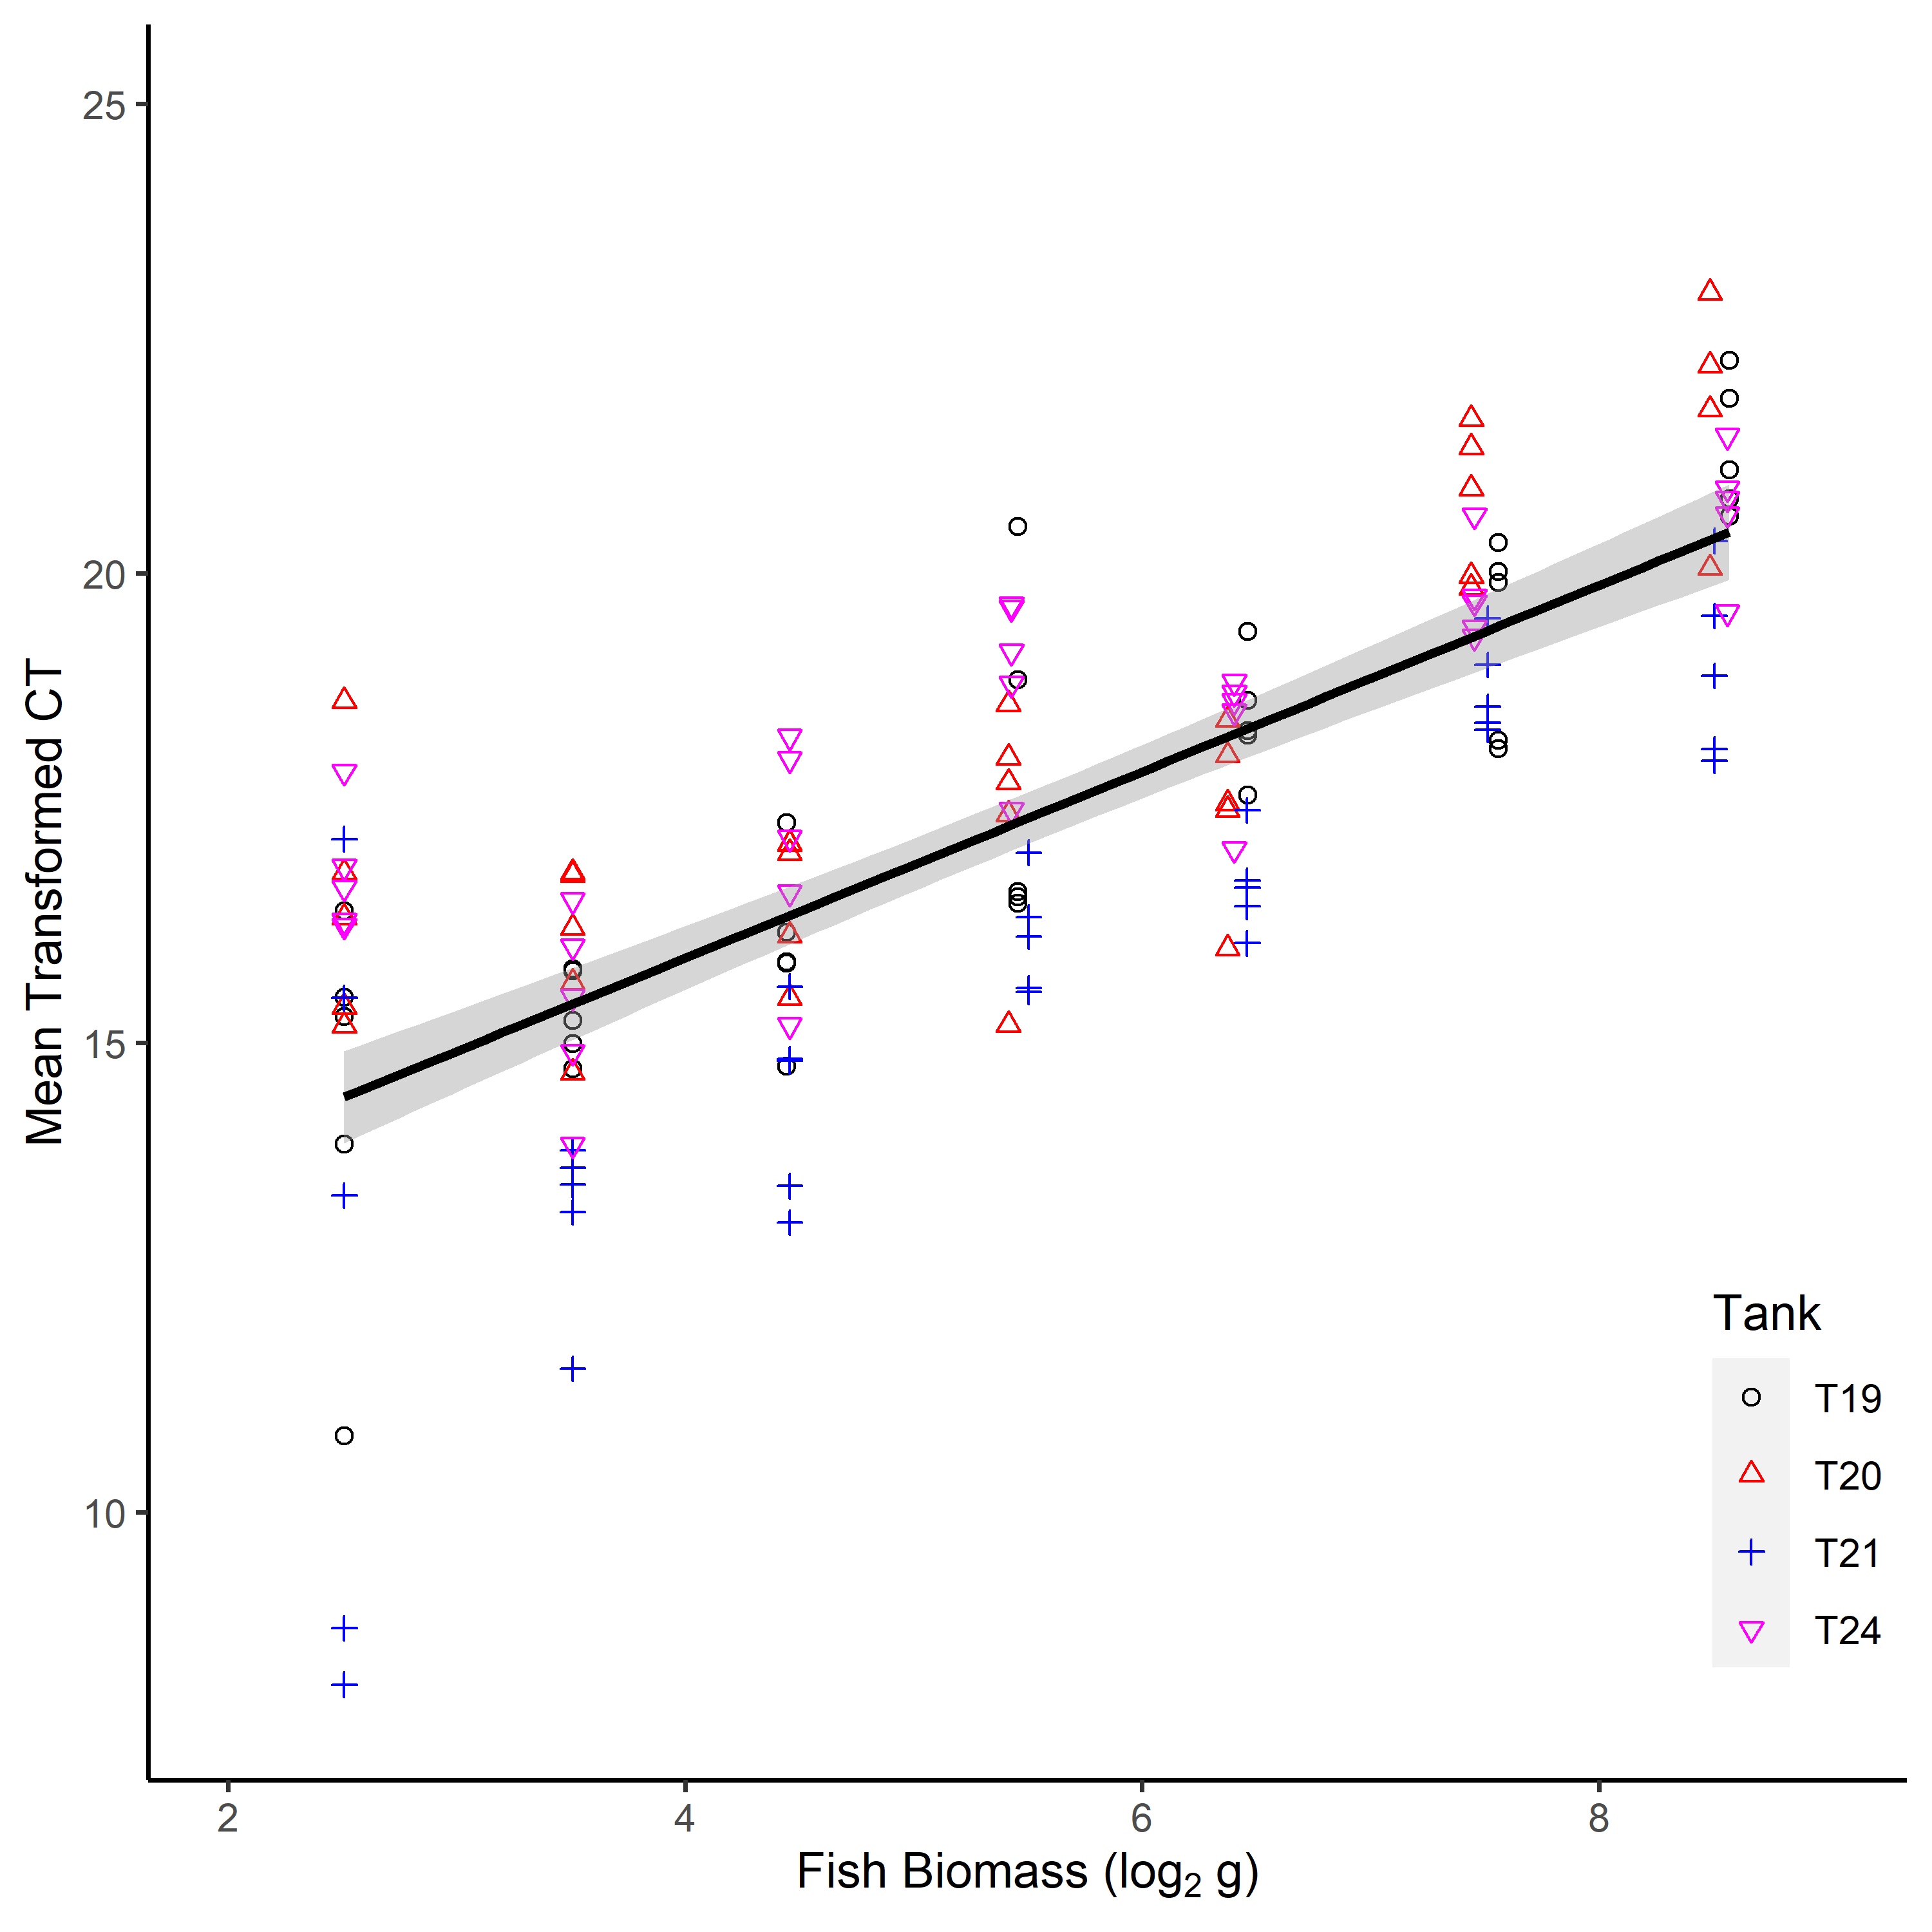
\includegraphics{Chapter3Images/ggplotnew3.png}
\caption{ \hspace{1mm}Mean TCT versus Log2(Biomass). The fitted regression line, l.one.line.mean and the 95 \% confidence intervals are included. Each of the four tanks has an associated color and shape.}
\label{fig:medct3}
\end{figure}

Figure~\ref{fig:medct3} plots l.one.line.mean and the associated 95 \% confidence bands.  Again, we see that the mean TCT from tank 21 tends to be less than the mean TCT from the other three tanks. In general, mean TCT increases as Log2(Biomass) increases.

\vspace{5mm}




\begin{table}[H]
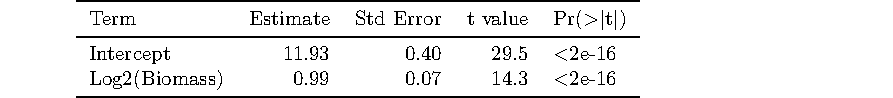
\includegraphics{Chapter3Images/lmMeanCorrect.pdf}
\caption{\hspace{1mm} Parameter estimates and standard errors for the model l.one.line.mean. This is a simple linear regression for mean TCT which only considers Log2(Biomass). The $R^{2}$ value is 0.692.}
\label{lab:loneline.mean}
\end{table}








Table~\ref{lab:loneline.mean} provides a summary of the parameter estimates for the simple linear model, l.one.line.mean. The estimates obtained are very similar to the estimates in Table~\ref{lab:loneline}.

\newpage

Next, we consider a model for mean TCT with biomass as a predictor, and also consider the impact of tank. We first plot regression lines obtained by considering a model with a common slope but allow for differing intercepts.

\begin{figure}[H]
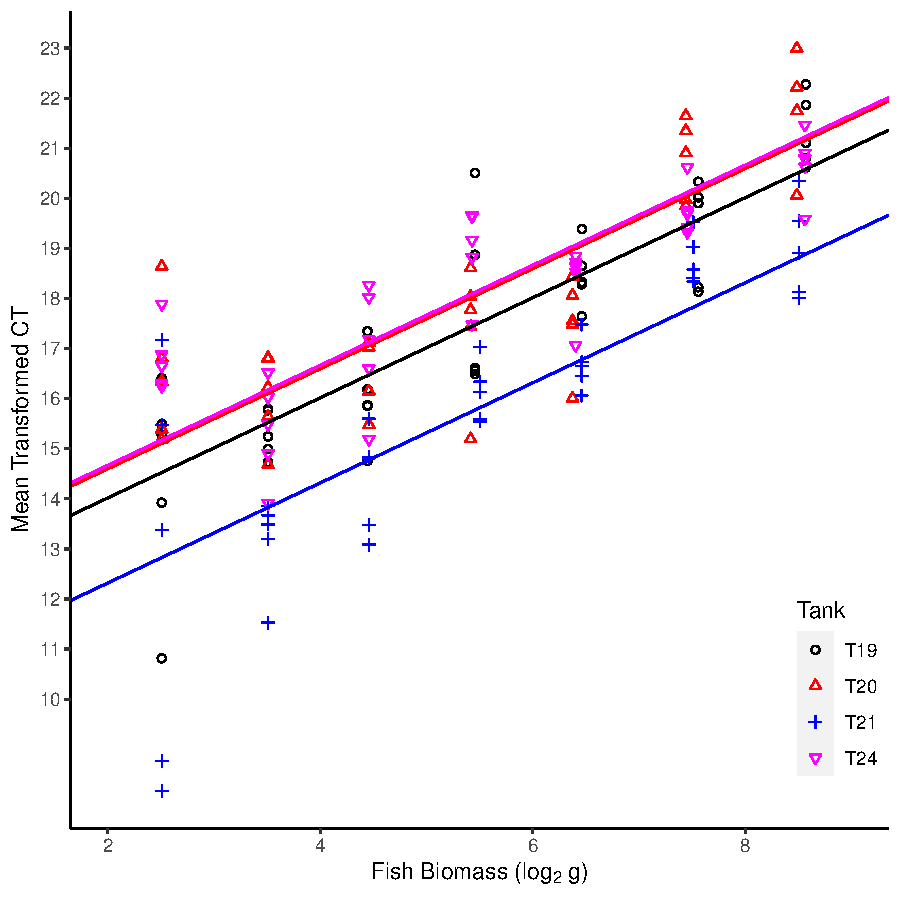
\includegraphics{Chapter3Images/parmean.pdf}
\caption{\hspace{1mm} Lines of best fit by allowing intercept to differ over each tank. This is a plot of the model lmparallel.tfac.mean.}
\label{fig:parmean}
\end{figure}









\begin{table}[H]
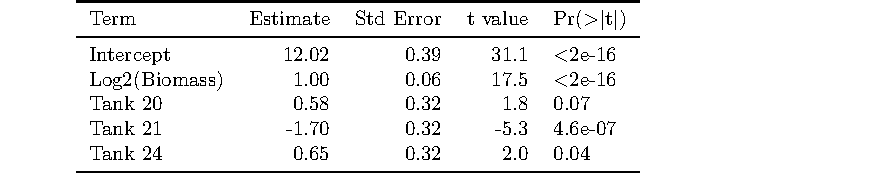
\includegraphics{Chapter3Images/lmMean2.pdf}
\caption{\hspace{1mm}Parameter estimates and standard errors for the model lmparallel.tfac.mean.This model allows for differing intercepts depending on which tank a sample came from. The $R^{2}$ value is 0.735.}
\label{lab:lmparallelmean}
\end{table}


Table~\ref{lab:lmparallelmean} summarizes the result of lmparallel.tfac.mean, which is a model including the tank as a predictor. The estimated intercept is 12.02 for lmparallel.tfac.mean, while the estimated intercept for the median TCT counterpart, lm.tfac was 12.36, which can be seen in Table~\ref{lab:lmparallel}.The effect of tank 21 is highly significant with an estimate of -1.7. That is, tank 21 produces much smaller mean TCT values compared to the other tanks.




\newpage

Finally, we built a full model, lfull.tfac.mean, that includes biomass, tank and the interactions between biomass and tank.

\begin{figure}[H]
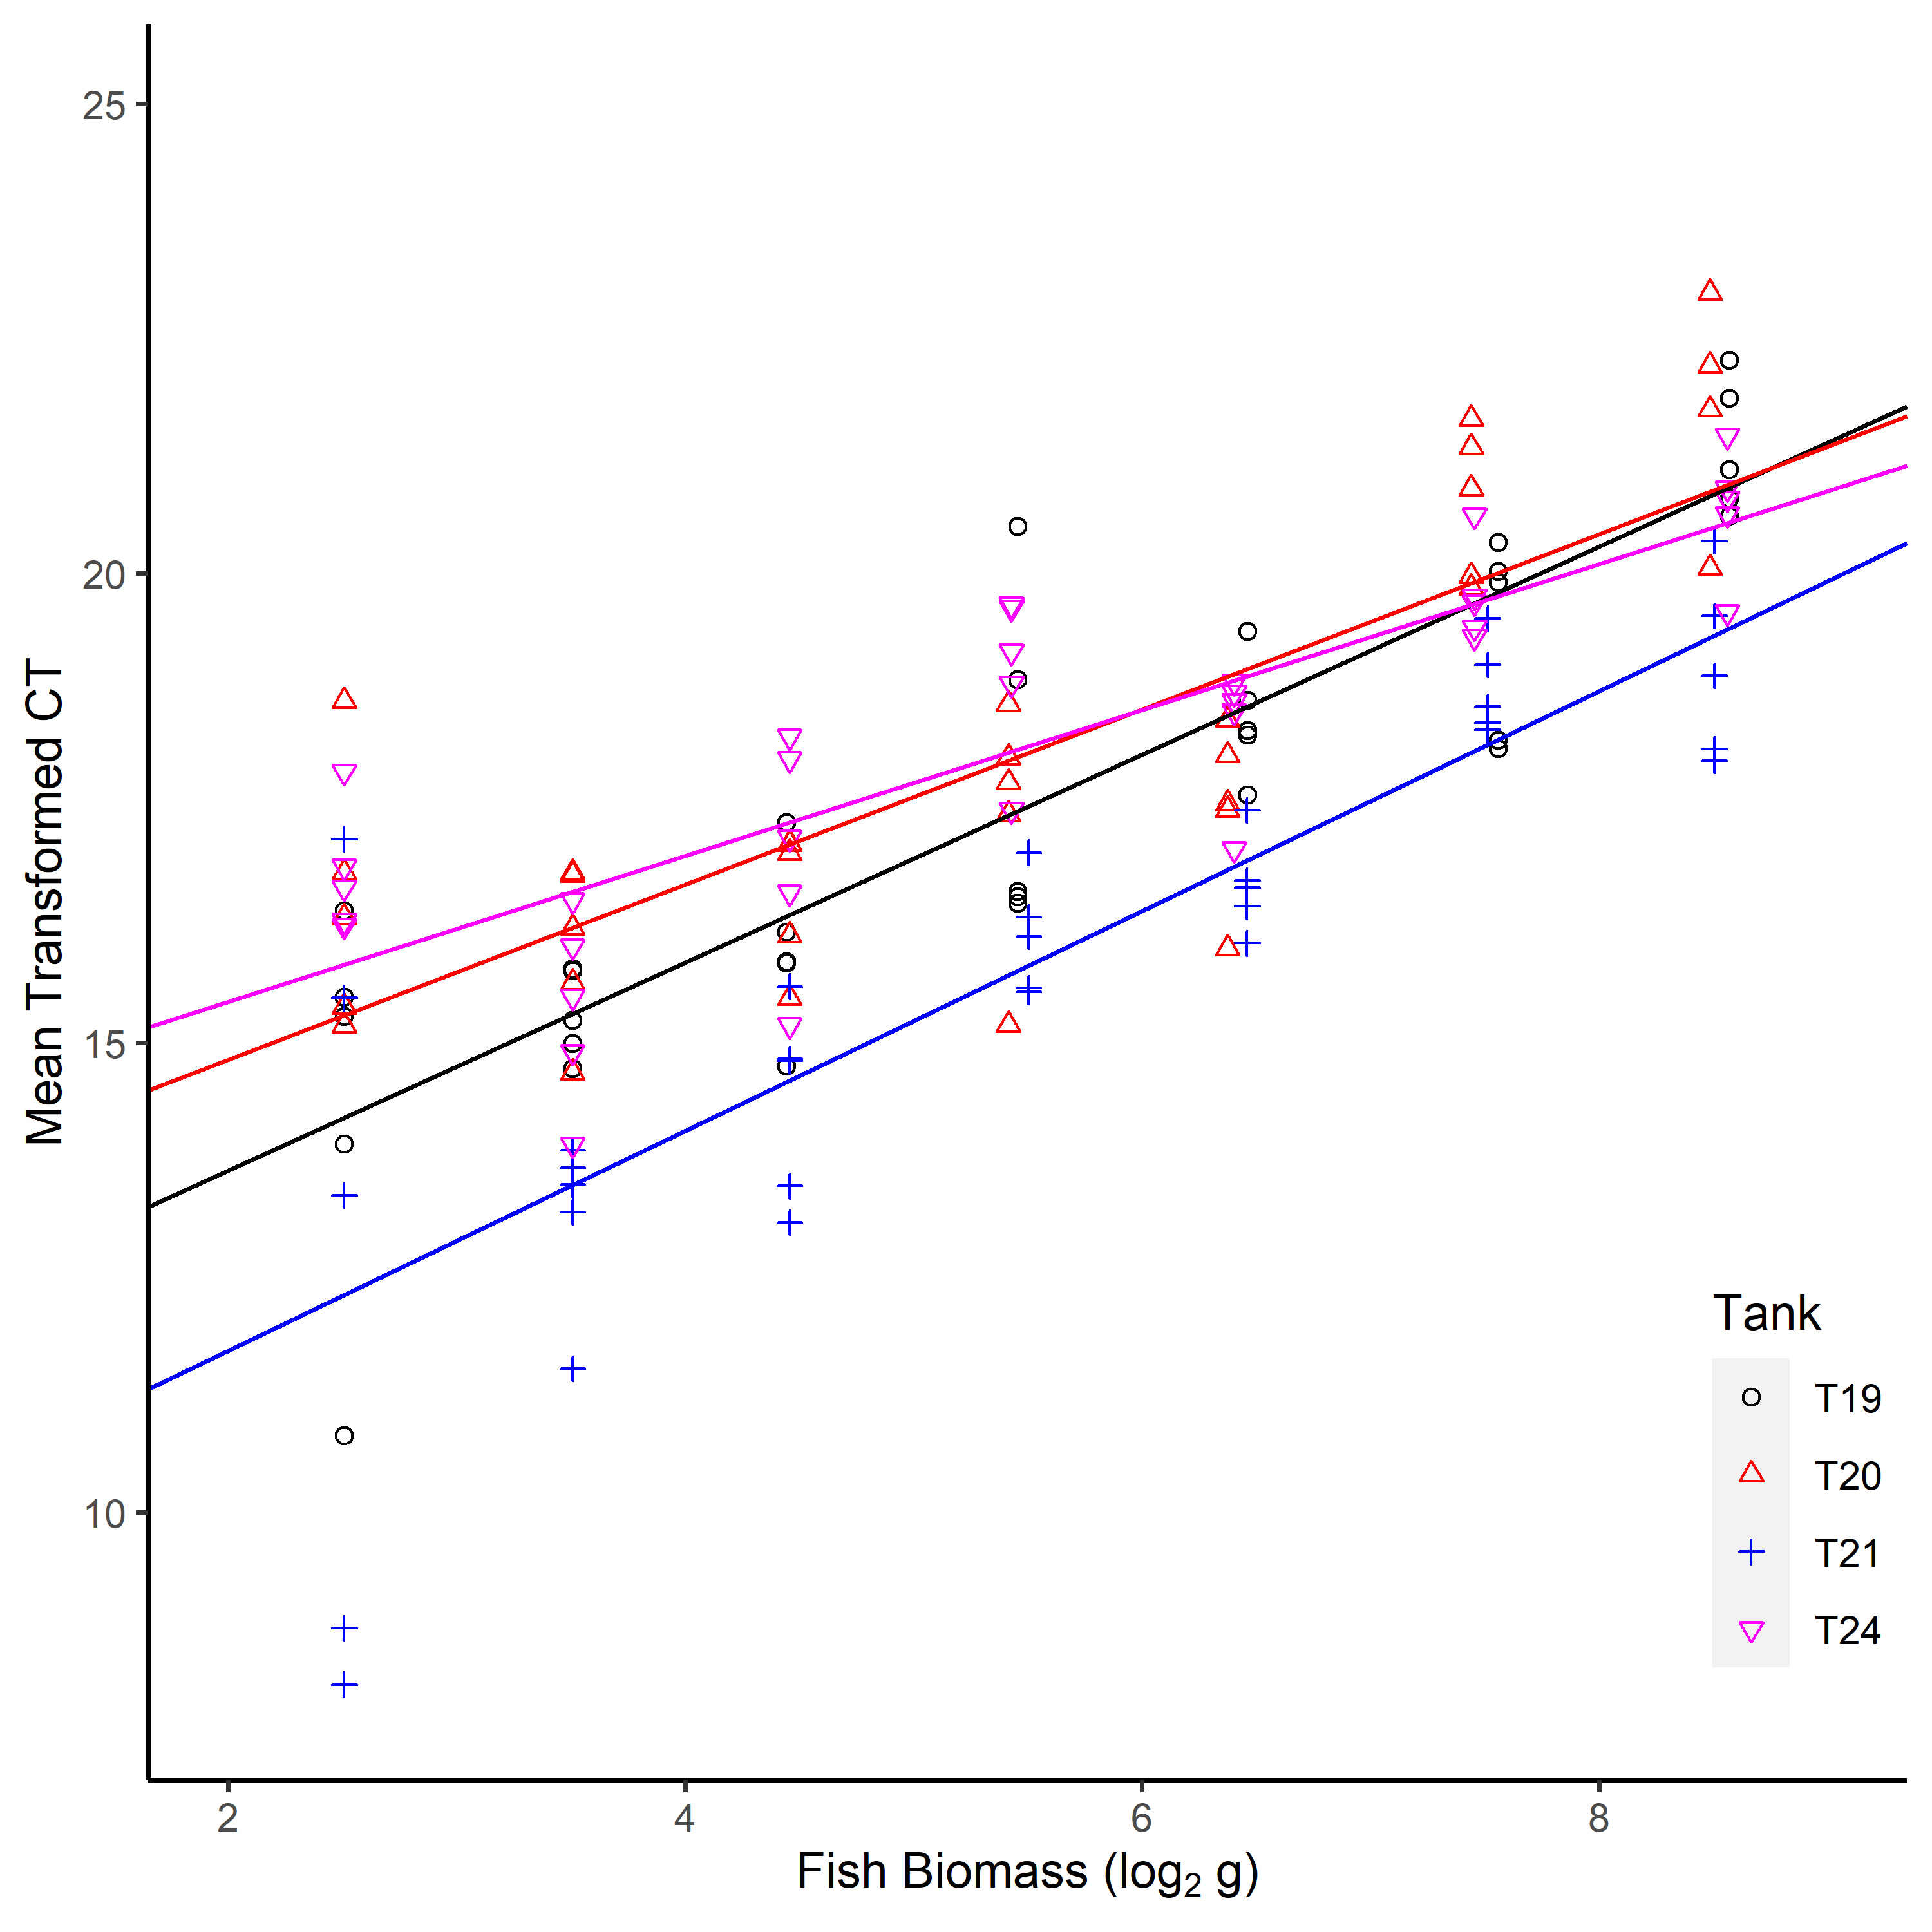
\includegraphics{Chapter3Images/ggplotnew7.png}
\caption{ \hspace{1mm}Lines of best fit by allowing intercept and slope to differ over each tank. This is a plot of the model lfull.tfac.mean.}
\label{fig:parmean}
\end{figure}


\begin{table}[H]
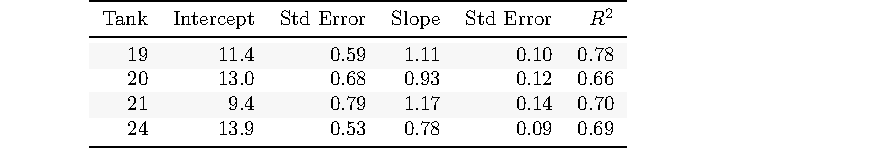
\includegraphics{Chapter3Images/meantankspecific.pdf}
\caption{Table summarizing simple linear regression on Log2(Biomass) when each tank is considered in isolation for mean TCT.}
\label{lab:sepmean}
\end{table}


Table~\ref{lab:sepmean} summarizes the results of applying simple linear regression to each tank in isolation. We obtained separate estimates for each intercept and slope. Tank 21 has the smallest intercept, while tank 24 has the largest intercept. The slopes are similar; however, tank 24 has a noticeably smaller slope. The $R^{2}$ are all quite high, but tank 19 alone has the highest $R^{2}$.







\begin{table}[H]
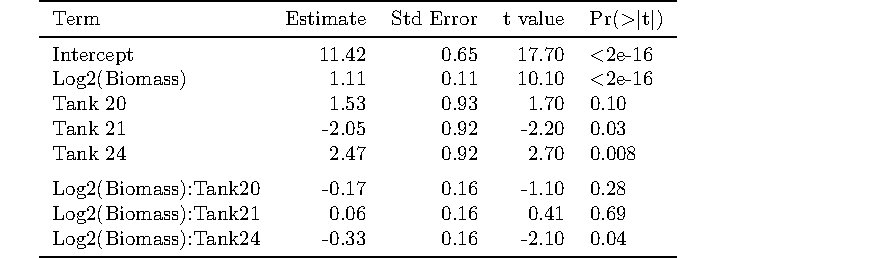
\includegraphics{Chapter3Images/lmMean3.pdf}
\caption{ \hspace{1mm}Parameter estimates and standard errors for a model that includes Log2(Biomass), tank and the interaction between tank and Log2(Biomass). Model:  lfull.tfac.mean. The $R^{2}$ value is 0.75.}
\label{fig:lfull2}
\end{table}


Figure~\ref{fig:parmean} is the plot of the model  lfull.tfac.mean. The intercept and slope is allowed to vary over each tank. Table~\ref{fig:lfull2} provides the summary of  lfull.tfac.mean. For the full model with mean TCT as the response and  both tank and the interaction between tank and biomass as predictors, the least squares estimate of the intercept term is 11.42. For the full model on median TCT, the least squares estimate of the intercept is 11.79. This model provides identical results to considering each tank in isolation, as seen by comparing the estimates to those given in Table~\ref{lab:sepmean}.

\newpage

We again create an ANOVA table:

   \vspace{12pt}




\begin{table}[H]
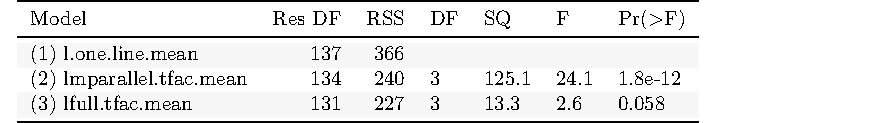
\includegraphics{Chapter3Images/anovamean.pdf}
\caption{\hspace{1mm}Summary of the additional sum of squares test for the Mean TCT models. }
\label{fig:anovamean11}
\end{table}


 
 Table~\ref{fig:anovamean11} shows the results of applying an ANOVA (additional sum of squares test) on the three models for Mean TCT. The interpretation is the same as it was with the anova table for median TCT. Since lmparallel.tfac.mean has a very small p-value, we conclude that we need to include the tank effect in our model (that is, we reject the hypothesis that differing intercepts is zero). 
Since the p-value associated with  lfull.tfac.mean is 0.058; this indicates that including interaction for modelling mean TCT is marginally significant (at the 0.05 level). The $R^{2}$ for lmparallel.tfac.mean is 0.735 while the $R^{2}$ for  lfull.tfac.mean is 0.750. Although the $R^{2}$ increases, it is only by a small amount. Since the p-value is on the boundary of significance, we may still choose to ignore the interaction term as it adds complexity and only slightly increases the $R^{2}$.

\newpage


We now fit a model similar to l.one.line.mean. However, we now collapse over each tank by taking the mean value of TCT. This model is called l.tankregression. Note this predictor, Log2(BiomassTank), is the Log2 taken over total weight in each of the four tanks.

 
\begin{figure}[H]
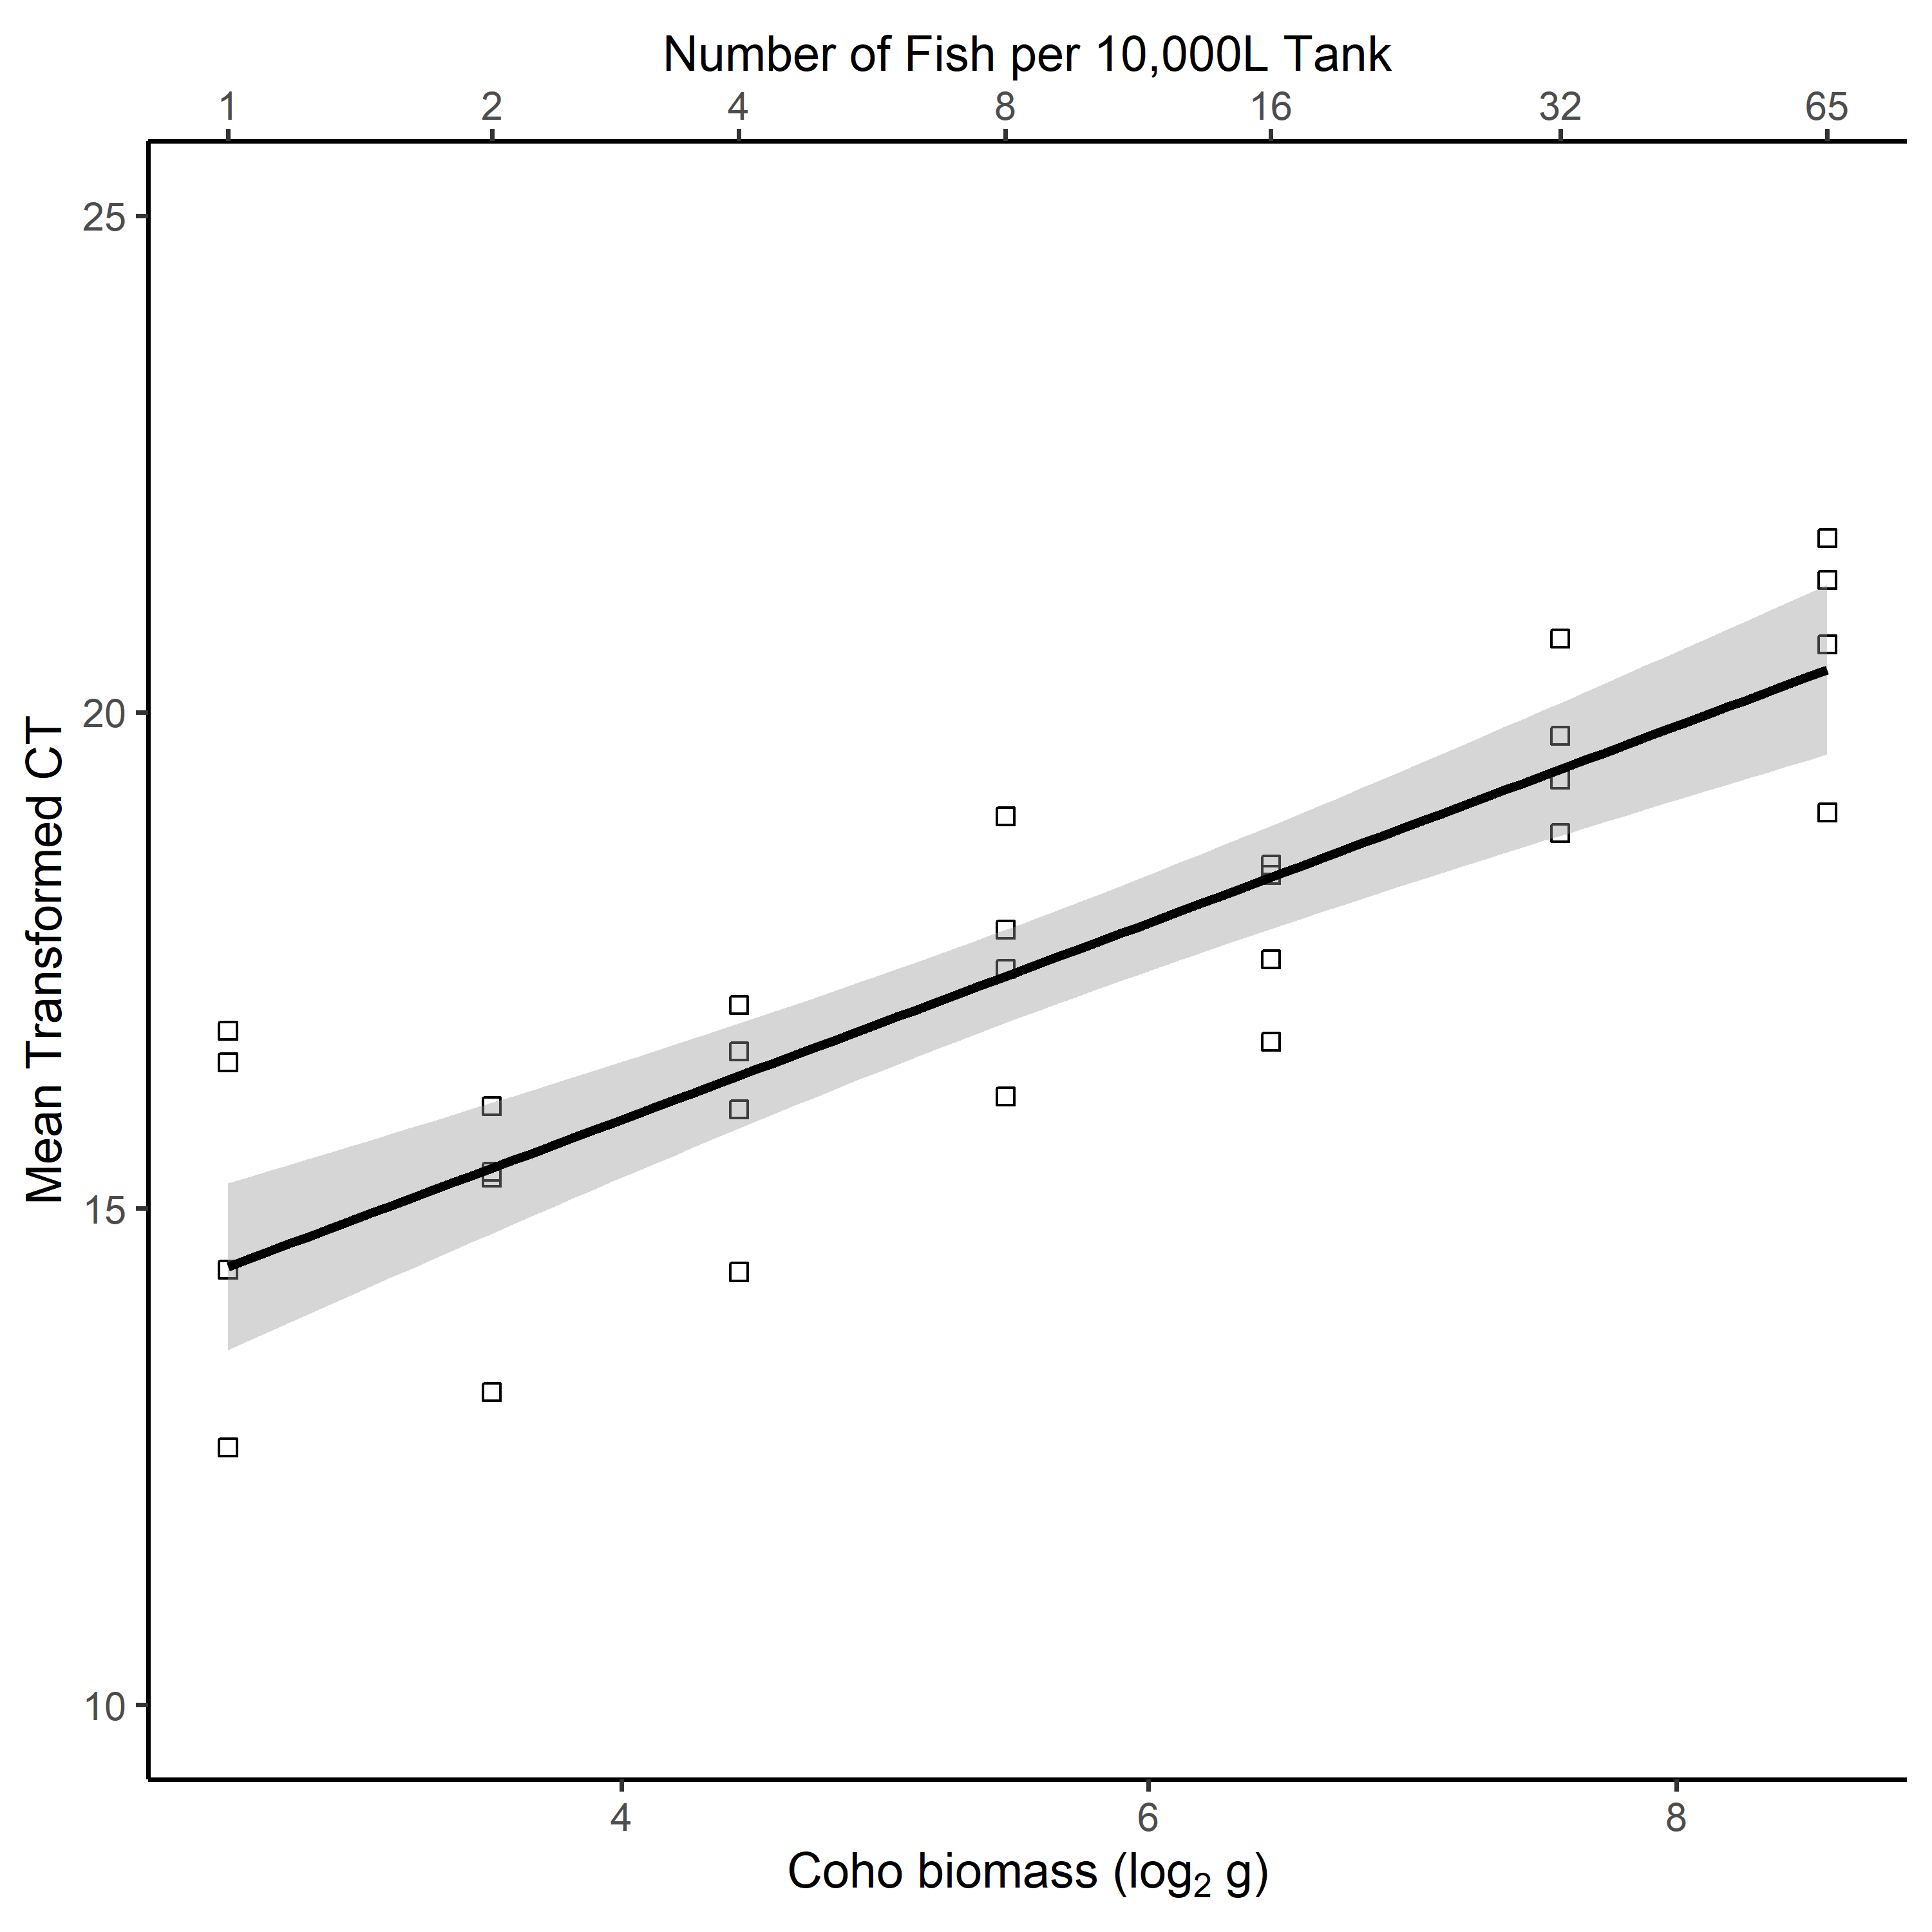
\includegraphics{Chapter3Images/ggplotnew4.png}
\caption{ \hspace{1mm} Regression line showing the relationship between Mean TCT and biomass. Included are the confidence bands about the regression line.  The line is the model l.tankregression. The $ R^{2}$ is 0.748. Points shown represent the Mean TCT for each of the four tanks for each of the seven unique numbers of fish.
}
\label{fig:medct55}
\end{figure}



\begin{table}[H]
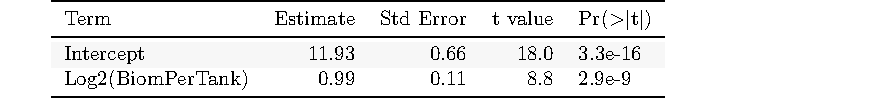
\includegraphics{Chapter3Images/tankregressionMEAN.pdf}
\caption{\hspace{1mm}Parameter estimates and standard errors for model: l.tankregression. The $R^{2}$ value is 0.748.}
\label{fig:lrankmean}
\end{table}

Table~\ref{fig:lrankmean} summarizes the result of taking the mean of TCT over each tank and fitting a simple regression model. The only variable considered is the Coho biomass. Figure~\ref{fig:medct55} is the regression line obtained by applying simple linear regression over the points collapsed by taking the mean over each tank. The $R^{2}$ is high, indicating our model does a good job at explaining variation in the data. Moreover, it has a simple interpretation (Mean TCT increases linearly with Log2(Biomass) and thus reduces complexity.




Figure~\ref{fig:medct55} is a plot made of our final model. Each point represents the Mean TCT for each of the four main tanks. Each distinct biomass value corresponds to a unique number of fish. 


